\begin{appendix}
\chapter{Anexo:Perfiles de las \'{A}reas Locales de g\_lomepro}\label{AnexoA}
En las figuras \ref{fig:apl_prof1},\ref{fig:apl_prof2} y \ref{fig:apl_prof3} se muestran las \'{a}reas por l\'{i}pido locales obtenidas para las r\'{e}plicas 1 a 3, para las dem\'{a}s r\'{e}plicas los resultados tienen la misma forma. La escala va de 0.55 a 0.79 y entre m\'{a}s rojo mayor es el \'{a}rea por l\'{i}pido. La escala para las membranas puras es de menor rango \ref{fig:apl_prof4}
\begin{figure}[ht]
\centering
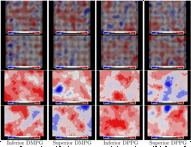
\includegraphics[resolution=400,scale=0.7]{Plots/glomepro/apl_glomepro_1.png}
\put(-150,90){15\%STX}
\put(-150,65){15\%STX}
\put(-150,40){1 STX}
\put(-150,20){1 STX}
\caption{\'{A}rea por l\'{i}pido locales para los sistemas con estafiloxantina. En la figura se muestra la monocapa superior y la inferior.}
\label{fig:apl_prof1}
\end{figure}
\begin{figure}[H]
\centering
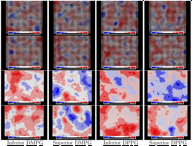
\includegraphics[resolution=400,scale=0.6]{Plots/glomepro/apl_glomepro_2.png}
\put(-132,75){15\%STX}
\put(-132,55){15\%STX}
\put(-132,35){1 STX}
\put(-132,15){1 STX}
\caption{\'{A}rea por l\'{i}pido locales para los sistemas con estafiloxantina. En la figura se muestra la monocapa superior y la inferior.}
\label{fig:apl_prof2}
\end{figure}
\begin{figure}[H]
\centering
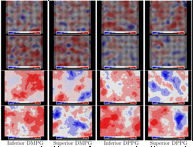
\includegraphics[resolution=400,scale=0.6]{Plots/glomepro/apl_glomepro_3.png}
\put(-132,75){15\%STX}
\put(-132,55){15\%STX}
\put(-132,35){1 STX}
\put(-132,15){1 STX}
\caption{\'{A}rea por l\'{i}pido locales para los sistemas con estafiloxantina. En la figura se muestra la monocapa superior y la inferior.}
\label{fig:apl_prof3}
\end{figure}
\begin{figure}[H]
\centering

\includegraphics[resolution=100,scale=0.8]{Plots/glomepro/apl_glomepro_mem.png}
% \put(-90,70){Inferior}
% \put(-70,70){Superior}
% \put(-50,70){Inferior}
% \put(-30,70){Superior}
\caption{\'{A}rea por l\'{i}pido locales para las membranas puras. En la figura se muestra la monocapa superior y la inferior.}
\label{fig:apl_prof4}
\end{figure}
%%%%%%%%%%%%%%%%%%%%%%%%%%%%%%%%%%%%%%%%%%%%%%%%%%%%%%%%%%%%%%%%%%%%%%%%%%%%%%%%%%%%%%%%%%%%%%%%%%%%%%%%%%%%%%%%%%%%%%
\chapter{Anexo:Perfiles de las Espesores Locales de g\_lomepro}\label{AnexoD}
En las figuras \ref{fig:thick_prof1},\ref{fig:thick_prof2} y \ref{fig:thick_prof3} se muestran los espesores locales obtenidas para las r\'{e}plicas 1 a 3, para las dem\'{a}s r\'{e}plicas los resultados tienen la misma forma. La escala va de 3.26 a 3.9$n$m y entre m\'{a}s rojo mayor es el espesor. La escala para las membranas puras es de menor rango \ref{fig:thick_prof4}: De 3.32 a 3.4 para DMPG y de 3.7 a 3.9 para DPPG.
\begin{figure}[ht]
\centering
\includegraphics[resolution=400,scale=0.7]{Plots/glomepro/join_plots/thick_glomepro_1.png}
\put(-150,90){15\%STX}
\put(-150,65){15\%STX}
\put(-150,40){1 STX}
\put(-150,20){1 STX}
\caption{Espesores locales para los sistemas con estafiloxantina. En la figura se muestra la monocapa superior y la inferior.}
\label{fig:thick_prof1}
\end{figure}
\begin{figure}[H]
\centering
\includegraphics[resolution=400,scale=0.6]{Plots/glomepro/join_plots/thick_glomepro_1.png}
\put(-132,75){15\%STX}
\put(-132,55){15\%STX}
\put(-132,35){1 STX}
\put(-132,15){1 STX}
\caption{Espesores locales para los sistemas con estafiloxantina. En la figura se muestra la monocapa superior y la inferior.}
\label{fig:thick_prof2}
\end{figure}
\begin{figure}[H]
\centering
\includegraphics[resolution=400,scale=0.6]{Plots/glomepro/join_plots/thick_glomepro_1.png}
\put(-132,75){15\%STX}
\put(-132,55){15\%STX}
\put(-132,35){1 STX}
\put(-132,15){1 STX}
\caption{Espesores locales para los sistemas con estafiloxantina. En la figura se muestra la monocapa superior y la inferior.}
\label{fig:thick_prof3}
\end{figure}
\begin{figure}[H]
\centering
\includegraphics[resolution=400,scale=0.7]{Plots/glomepro/join_plots/thick_glomepro_mem.png}
% \put(-90,70){Inferior}
% \put(-70,70){Superior}
% \put(-50,70){Inferior}
% \put(-30,70){Superior}
\caption{Espesores locales para las membranas puras. En la figura se muestra la monocapa superior y la inferior.}
\label{fig:thick_prof4}
\end{figure}
%%%%%%%%%%%%%%%%%%%%%%%%%%%%%%%%%%%%%%%%%%%%%%%%%%%%%%%%%%%%%%%%%%%%%%%%%%%%%%%%%%%%%%%%%%%%%%%%%%%%%%%%%%%%%%%%%%%%%%
\chapter{Anexo: Perfiles de Estr\'{e}s sin Filtrar}\label{AnexoB}
A continuaci\'{o}n se muestran los perfiles de estr\'{e}s promediados sin filtrar y promediado entre las 5 r\'{e}plicas realizadas por cada sistema.
En la figura \ref{fig:stress0} derecha aparece el perfil de estr\'{e}s al aplicar un filtro gaussiano de 4 desviaciones est\'{a}ndar.\\
%trim={<left> <lower> <right> <upper>}
\begin{figure}[h]
\begin{center}
    \includegraphics[scale=0.22,trim={0 6cm 0 8cm},clip]{Plots/stress_profile.png}
        \includegraphics[scale=0.22,trim={0 6cm 0 8cm},clip]{Plots/stress_profile_4.png}
  \caption{\textit{Izquierda}: Perfil de estr\'{e}s promediado para todas las r\'{e}plicas y sin filtrar.\textit{Derecha}: Perfil de estr\'{e}s con un filtro gaussiano de 4. }
  \label{fig:stress0}
\end{center}
\end{figure}

% \begin{figure}[H]
% \begin{center}
%     \includegraphics[scale=0.25]{Plots/stress_profile_4.png}
%   \caption{Perfil de estr\'{e}s promediado para todas las r\'{e}plicas y sin filtrar. }
%   \label{fig:stress2_a}
% \end{center}
% \end{figure}
\chapter{Anexo: MSD y Coeficientes de Difusi\'{o}n para Todos los Sistemas}\label{AnexoC}
En las figuras \ref{fig:msdlipid} y \ref{fig:msdstx} aparecen las fluctuaciones cuadr\'{a}ticas medias para los l\'{i}pidos y para la estafiloxantina respectivamente. Estas fueron obtenidas con la herramienta gromacs, en la cual se calcul\'{o} la fluctuaci\'{o}n por cada mol\'{e}cula partiendo de la conformaci\'{o}n a los $150n$s y luego se promedi\'{o} la fluctuaci\'{o}n para todas las macromol\'{e}culas de la misma especie. En el caso de las estafiloxantinas se tomaron ventanas de tiempo m\'{a}s cortas de $40n$s.
\begin{figure}[h]
\begin{center}
    \includegraphics[scale=0.28,trim={0 2cm 0 6cm},clip]{Plots/msd_stx_40.png}
  \caption{Desviaciones cuadr\'{a}ticas medias de STX utilizadas para hallar el coeficiente de difusi\'{o}n. Cada color es por cada r\'{e}plica. Se han descartado los primeros $100n$s para realizar el ajuste y se han escogido ventanas de $40n$s.}
  \label{fig:msdstx}
\end{center}
\end{figure}
\begin{figure}[ht]
\begin{center}
    \includegraphics[scale=0.28,trim={0 3cm 0 4cm},clip]{Plots/msd_lipid_40.png}
  \caption{Desviaciones cuadr\'{a}ticas medias de los l\'{i}pidos utilizadas para hallar el coeficiente de difusi\'{o}n. Cada color es por cada r\'{e}plica. Se han descartado los primeros $100n$s para realizar el ajuste y se han escogido ventanas de $40n$s.}
  \label{fig:msdlipid}
\end{center}
\end{figure}
%%%%%%%%%%%%%%%%%%%%%%%%%%%%%%%%
\begin{sidewaystable}% 
\centering
\begin{tabular}{|c|c|c|c|c|}
\toprule
{} &   $  D_{STX}((\mu\mathrm{m})^ 2\mathrm{s^ {-1}})$ &   $   D_{Lipid} ((\mu\mathrm{m})^ 2s^ {-1})$ &   $  D_{STX} 40ns  ((\mu\mathrm{m})^ 2\mathrm{s^ {-1}})$ &    $  D_{Lipid}40ns  (\mu\mathrm{m^ 2s^ {-1}})$ \\
\midrule
\textbf{15STX-DMPG     } & 7.9 & 9.1 & 5.3 & 6.5 \\
\textbf{15STX-DPPG     } & 5.8 & 7.0 & 4.0 & 5.6 \\
\textbf{15STXrigid-DMPG} & 6.8 & 8.1 & 4.7 & 6.2 \\
\textbf{15STXrigid-DPPG} & 5.7 & 6.9 & 4.0 & 5.6 \\
\textbf{MEM-DMPG       } & NaN &12.6 & NaN &14.3 \\
\textbf{MEM-DPPG       } & NaN &15.2 & NaN &16.7 \\
\textbf{STX-DMPG       } &16.0 &16.6 & 7.2 &10.4 \\
\textbf{STX-DPPG       } &13.4 &13.7 & 9.0 &12.6 \\
\textbf{STXrigid-DMPG  } &14.2 &18.5 & 8.8 &15.2 \\
\textbf{STXrigid-DPPG  } &11.9 &14.6 & 2.1 & 6.8 \\
\bottomrule
\end{tabular}
\caption{Coeficientes de difusi\'{o}n para una caja finita en condiciones de frontera peri\'{o}dicas. Las columnas con que dicen $40n$s son en las que se han tomado ventanas de tiempo de $40n$s y las otras donde se ha tomado la trayectoria de $100n$s a $400n$s.}
    \label{tab:dpbc}
\end{sidewaystable}
%%%%%%%%%%%%%%%%%%%%%%%%%%%%%%%%%%%%%
\begin{sidewaystable}
    \centering
\begin{tabular}{|c|c|c|c|c|}
\toprule
{} &   $  D_{STX}((\mu\mathrm{m})^ 2\mathrm{s^ {-1}})$ &   $   D_{Lipid} ((\mu\mathrm{m})^ 2s^ {-1})$ &   $  D_{STX} 40ns  ((\mu\mathrm{m})^ 2\mathrm{s^ {-1}})$ &    $  D_{Lipid}40ns  (\mu\mathrm{m^ 2s^ {-1}})$ \\
\midrule
\textbf{15STX-DMPG     } &10.4 &11.6 & 7.9 & 9.1 \\
\textbf{15STX-DPPG     } &51.8 &53.0 &50.1 &51.6 \\
\textbf{15STXrigid-DMPG} & 9.3 &10.7 & 7.2 & 8.8 \\
\textbf{15STXrigid-DPPG} &51.7 &52.9 &49.9 &51.6 \\
\textbf{MEM-DMPG       } & NaN &16.1 & NaN &17.8 \\
\textbf{MEM-DPPG       } & NaN &78.9 & NaN &80.4 \\
\textbf{STX-DMPG       } &19.2 &19.8 &10.4 &13.5 \\
\textbf{STX-DPPG       } &68.7 &69.0 &64.3 &67.9 \\
\textbf{STXrigid-DMPG  } &17.4 &21.7 &12.0 &18.3 \\
\textbf{STXrigid-DPPG  } &67.2 &69.8 &57.3 &62.1 \\
\bottomrule
\end{tabular}
    \caption{Coeficientes de difusi\'{o}n para una caja infinita halladas con la correcci\'{o}n de \cite{Vogele2016DivergentMembranes}. Las columnas con que dicen $40n$s son en las que se han tomado ventanas de tiempo de $40n$s y las otras donde se ha tomado la trayectoria de $100n$s a $400n$s.}
    \label{tab:dinf}
\end{sidewaystable}
% \chapter{Anexo: Nombrar el anexo C de acuerdo con su contenido}
% MANEJO DE LA BIBLIOGRAF\'{I}A: la bibliograf\'{\i}a es la relaci\'{o}n de las fuentes documentales consultadas por el investigador para sustentar sus trabajos. Su inclusi\'{o}n es obligatoria en todo trabajo de investigaci\'{o}n. Cada referencia bibliogr\'{a}fica se inicia contra el margen izquierdo.\\

% La NTC 5613 establece los requisitos para la presentaci\'{o}n de referencias bibliogr\'{a}ficas citas y notas de pie de p\'{a}gina. Sin embargo, se tiene la libertad de usar cualquier norma bibliogr\'{a}fica de acuerdo con lo acostumbrado por cada disciplina del conocimiento. En esta medida es necesario que la norma seleccionada se aplique con rigurosidad.\\

% Es necesario tener en cuenta que la norma ISO 690:1987 (en Espa\~{n}a, UNE 50-104-94) es el marco internacional que da las pautas m\'{\i}nimas para las citas bibliogr\'{a}ficas de documentos impresos y publicados. A continuaci\'{o}n se lista algunas instituciones que brindan par\'{a}metros para el manejo de las referencias bibliogr\'{a}ficas:\\

% \begin{center}
% \centering%
% \begin{tabular}{|p {7.5 cm}|p {7.5 cm}|}\hline
% \arr{Instituci\'{o}n}&Disciplina de aplicaci\'{o}n\\\hline%
% Modern Language Association (MLA)&Literatura, artes y humanidades\\\hline%
% American Psychological Association (APA)&Ambito de la salud (psicolog\'{\i}a, medicina) y en general en todas las ciencias sociales\\\hline
% Universidad de Chicago/Turabian &Periodismo, historia y humanidades.\\\hline
% AMA (Asociaci\'{o}n M\'{e}dica de los Estados Unidos)&Ambito de la salud (psicolog\'{\i}a, medicina)\\\hline
% Vancouver &Todas las disciplinas\\\hline
% Council of Science Editors (CSE)&En la actualidad abarca diversas ciencias\\\hline
% National Library of Medicine (NLM) (Biblioteca Nacional de Medicina)&En el \'{a}mbito m\'{e}dico y, por extensi\'{o}n, en ciencias.\\\hline
% Harvard System of Referencing Guide &Todas las disciplinas\\\hline
% JabRef y KBibTeX &Todas las disciplinas\\\hline
% \end{tabular}
% \end{center}

% Para incluir las referencias dentro del texto y realizar lista de la bibliograf\'{\i}a en la respectiva secci\'{o}n, puede utilizar las herramientas que Latex suministra o, revisar el instructivo desarrollado por el Sistema de Bibliotecas de la Universidad Nacional de Colombia\footnote{Ver: www.sinab.unal.edu.co}, disponible en la secci\'{o}n "Servicios", opci\'{o}n "Tr\'{a}mites" y enlace "Entrega de tesis".

\end{appendix}